\chapter {Prophet}

\section {Despre Prophet}

\noindent Prophet \cite{prophet} este un model open-source dezvoltat de Facebook pentru analiza seriilor de timp, \^ in special pentru prognozare (``forecasting"). Aceast\u a libr\u arie separ\u a componentele de trend, sezoniere \c si reziduale, folosind \^ in spate regresie non-liniar\u a. Descompunerea seriei de timp se face \^ in felul urm\u ator: 

$$ y(t) = g(t) + s(t) + h(t) + \epsilon_t$$

unde $y$ este seria complet\u a de timp, $g$ este func\c tia de trend, $s$ este func\c tia de sezonalitate, $h$ este func\c tia care modeleaz\u a efectele vacan\c telor ce pot ap\u area \^ in mod neregulat asupra uneia sau mai multor zile, iar $\epsilon_t$ este termenul de eroare rezidual\u a \cite{prophet}. \\

%\noindent Prin arhitectura sa, acest model face prognoze analiz\^ and \^ intreaga serie de timp. Totu\c si, poate fi adaptat s\u a fac\u a detec\c tia unei anomalii doar \^ in ultimul punct, \^ intr-un mod care nu este foarte eficient, a\c sa cum este detaliat \^ in capitolul urm\u ator. \\

\section {Formatul predic\c tiilor}

\noindent Din punct de vedere al predic\c tiilor, pentru fiecare punct din prognoza generat\u a de Prophet, avem $3$ valori: \texttt{yhat}, \texttt{yhat\_lower} \c si \texttt{yhat\_upper}. Ultimele dou\u a valori reprezint\u a limitele intervalului de incertitudine, \^ in timp ce \texttt{yhat} este valoarea estimat\u a pe baza acestor valori. Pe baza datelor din trecut, am calculat o eroare absolut\u a (diferen\c ta dintre valoarea actual\u a si cea prezis\u a), respectiv un factor de incertitudine (diferen\c ta \^ intre capetele intervalului de incertitudine). Am considerat anomalii acele puncte pentru care eroarea era mai mare dec\^ at pragul de incertitudine, \^ inmul\c tit cu un factor setat. \\

\section {G\u asirea factorului optim, rezultate \c si concluzii}

\noindent Prima \^ incercare a fost aplicarea metodei procentuale pe Prophet, dar aceasta nu a mers pentru c\u a este func\c tional\u a doar dac\u a num\u arul de anomalii depinde monoton de un singur parametru. \^ In continuare, factorul a fost determinat din mai multe rul\u ari (\c si rezultatele cele mai bune au fost ob\c tinute pe intervalul $\interval{1.25}{1.5}$, i.e o eroare mai mare cu $25\%$ - $50\%$ dec\^ at intervalul de incertitudine). \\

\noindent Totodat\u a, pentru a stabili relevan\c ta rezultatelor ob\c tinute din aceste rul\u ari, am ales mai multe instrumente financiare, cu diverse volatilit\u a\c ti si sezonalit\u a\c ti, select\^ andu-le cu ajutorul indicatorului $\beta$. Am comparat rezultatele ob\c tinute de Prophet pentru detectarea de anomalii cu ajutorul a trei instrumente: Ethereum (este cunoscut faptul c\u a pe pia\c ta de criptomonede volatilitatea este mult mai mare), AAPL (o ac\c tiune cu volatilitate medie, av\^ and $\beta = 1.29$ la momentul redact\u arii) \c si VZ (o ac\c tiune cu volatilitate mic\u a, av\^ and $\beta = 0.38$ la momentul redact\u arii). Graficile prezentate arat\u a ultimii 5 ani din seriile de timp, dar Prophet a fost antrenat cu \^ intreg setul de date disponibil pe Yahoo Finance. \\

\noindent Din punct de vedere al m\u asur\u arii erorilor, modelul a ob\c tinut rezultate foarte bune, ob\c tin\^ and valoarea erorii mediii absolute procentuale \^ in jurul valorilor $0.1\%$ - $0.2\%$ \^ in cazul ac\c tiunilor \c si \^ in jur de $1\%$ pentru criptomonede. 

\begin{wrapfigure}[16]{r}{0.5\textwidth}
%\begin{center}
    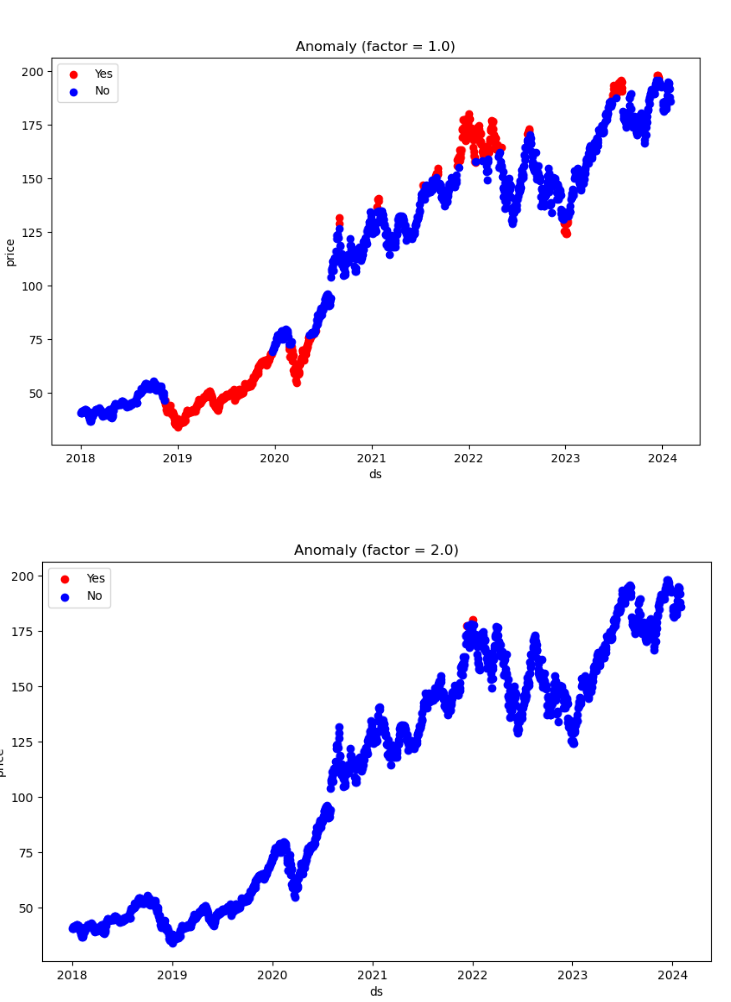
\includegraphics[width=0.48\textwidth]{apple_12.png}
  %\end{center}
\end{wrapfigure}

\hfill \break 

\noindent Am \^ inceput prin a selecta valorile $1$ \c si $2$ pentru factor pe ac\c tiunea AAPL, pentru a vedea cum se comport\u a modelul. \\ \\ A\c sa cum reiese din grafice, pentru valoarea $1$ a detectat multe valori ca anomalii, \^ in timp ce pentru valoarea $2$ a detectat una singur\u a, pe v\^ arful de la sf\^ ar\c situl anului 2021. Prin urmare, pentru a verifica dac\u a factorul $2$ este \^ intr-adev\u ar prea mare pentru ca modelul s\u a detecteze anomalii, am ales un instrument mult mai volatil, \c si anume ETH-USD (Ethereum).

\newpage 

\noindent Chiar \c si \^ in acest caz, detectarea anomaliilor este una redus\u a pentru un instrument at\^ at de volatil, a\c sa c\u a urm\u atoarul experiment a implicat rularea ambelor instrumente cu factorul $1.5$. 

\begin{wrapfigure}[16]{l}{0.5\textwidth}
%\begin{center}
    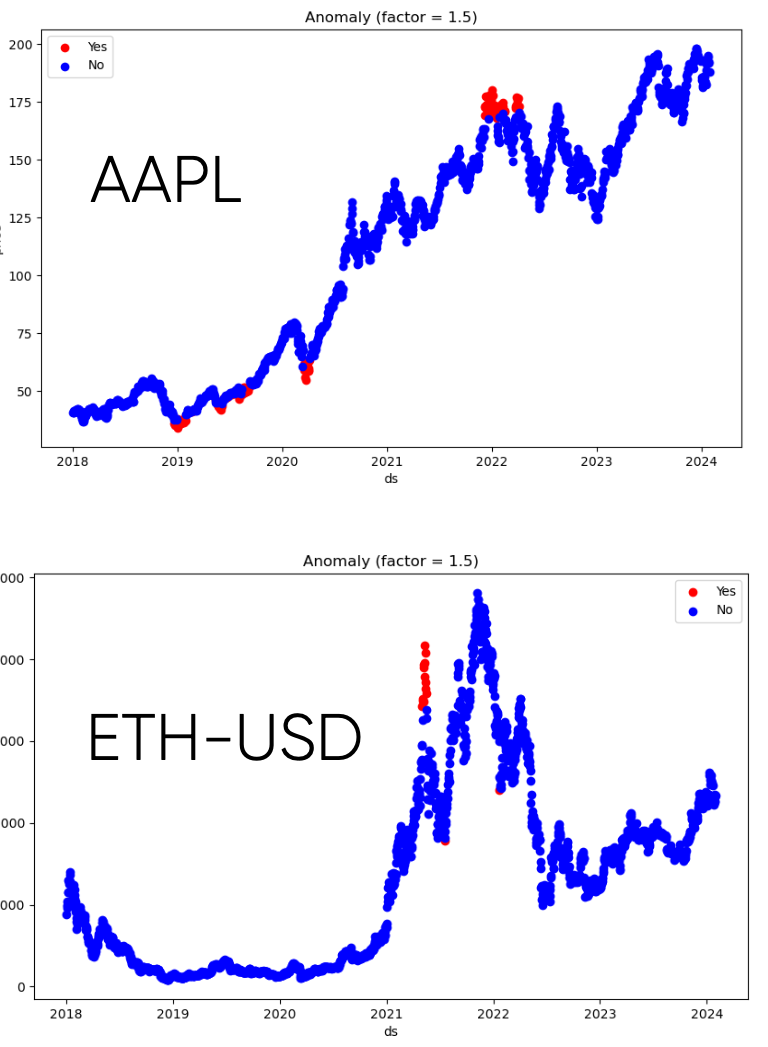
\includegraphics[width=0.48\textwidth]{15.png}
  %\end{center}
\end{wrapfigure}

\hfill \break

\noindent Se poate observa c\u a modelul \^ incepe s\u a dea rezultate de o calitate mai bun\u a, detect\^ and mai multe puncte de minim \c si mai multe de maxim (puncte ce sunt bune pentru efectuare de tranza\c tii de long, respectiv short, \^ in contextul unui program de trading algoritmic). \\
\noindent Aceast\u a valoare este una bun\u a, a\c sa c\u a urmeaz\u a s\u a fie validat\u a \c si pentru ac\c tiunea VZ. Totodat\u a, pentru a verifica dac\u a o valoare mai mic\u a poate ob\c tine rezultate mai bune, este nevoie de o rulare pe toate cele trei instrumentele folosite p\^ ana acum, cu valoarea factorului de $1.25$. 

\begin{wrapfigure}[5]{r}{0.5\textwidth}
%\begin{center}
    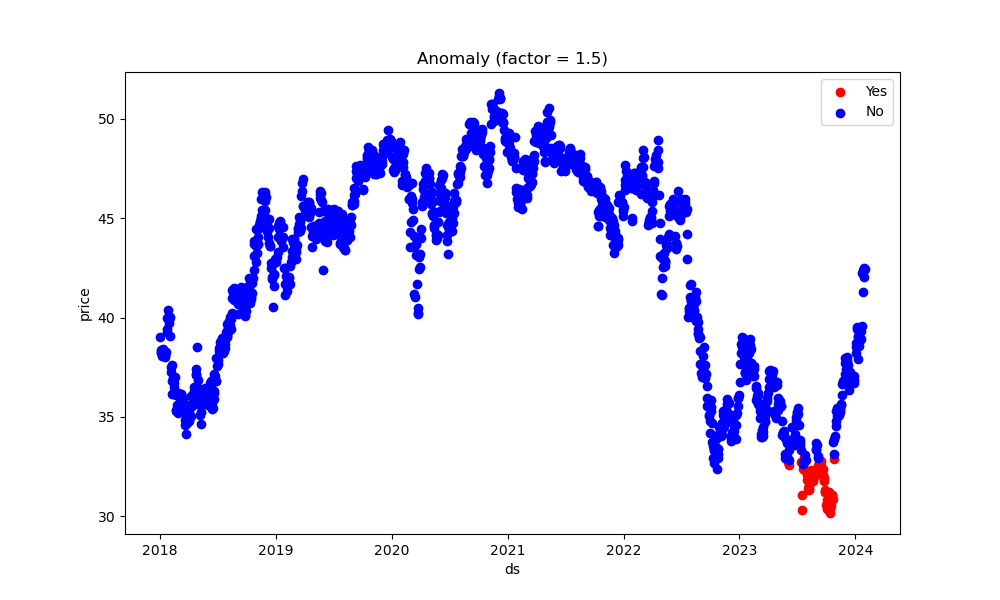
\includegraphics[width=0.48\textwidth]{VZ_1.5.png}
  %\end{center}
\end{wrapfigure}

\hfill \break 

\noindent Rezultatele ob\c tinute pentru VZ (imaginea din dreapta) confirm\u a faptul c\u a $1.5$ este un factor bun. Av\^ and $\beta$ mic, este de a\c steptat ca anomaliile detectate s\u a fie mai pu\c tine. 

\hfill \break 

\begin{center} 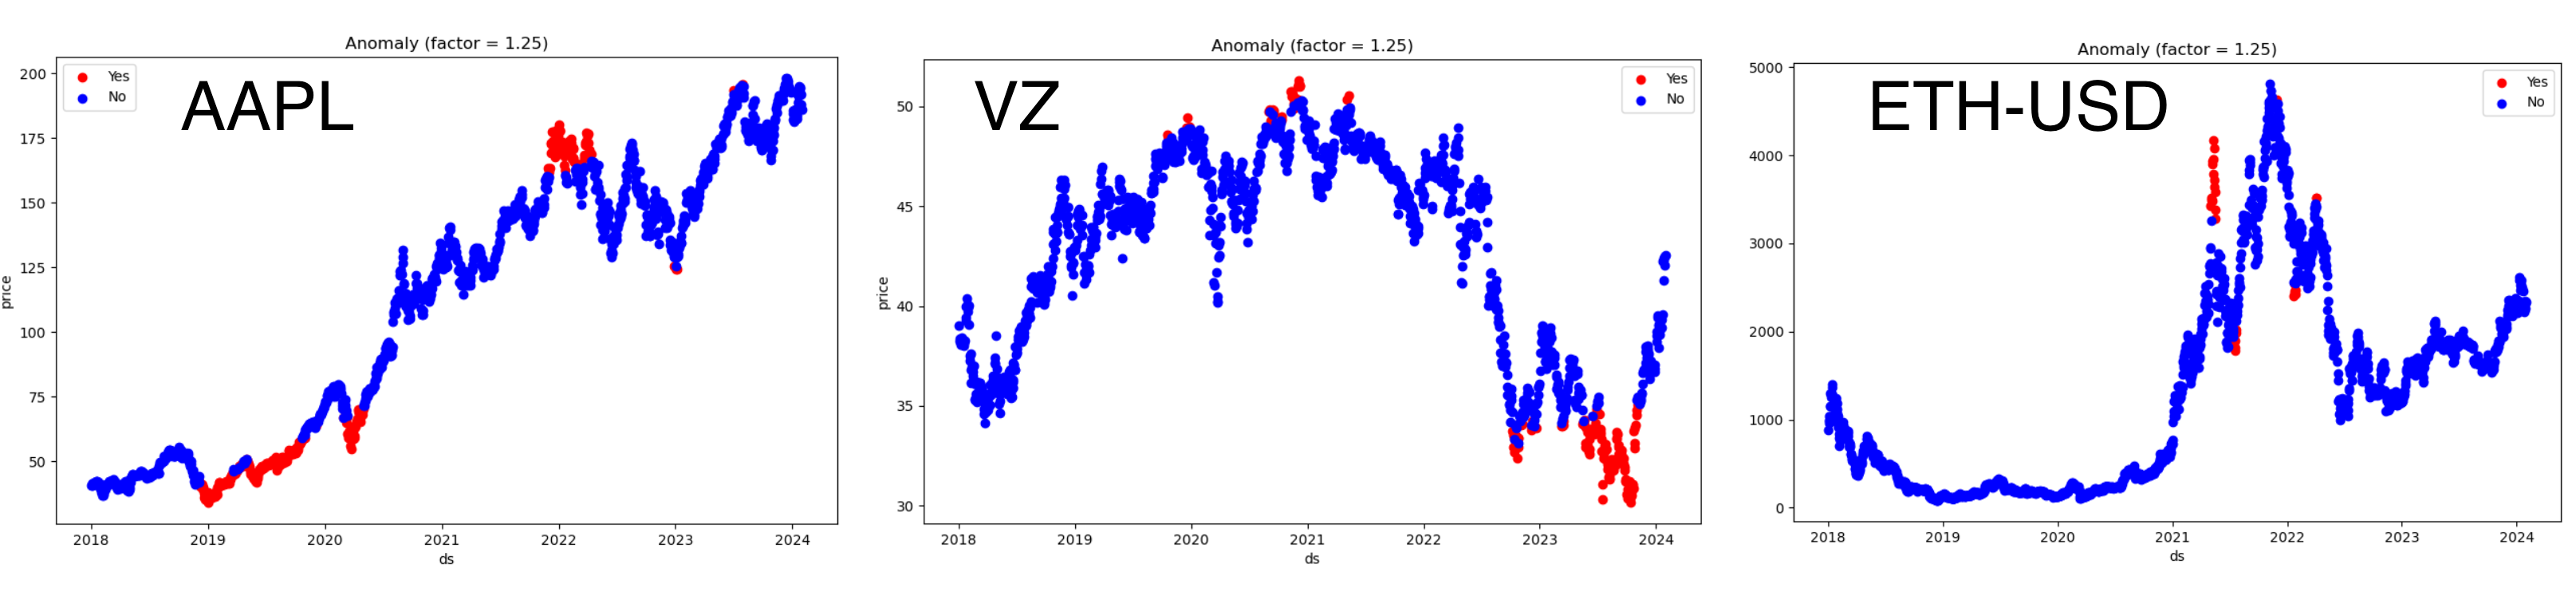
\includegraphics[width=\textwidth]{125.png} \end{center}

\noindent \c Si pentru factorul $1.25$ au fost ob\c tinute rezultate foarte bune, dar, \^ in mod evident, modelul este mai sensibil \c si va detecta mai multe anomalii. Prin urmare, \^ in functie de comportamentul a\c steptat de c\u atre utilizator, acest prag poate fi situat \^ intre $1.25$ \c si $1.5$. 